\documentclass[border=10pt]{standalone}

\usepackage{tikz}
\usepackage{tikzsymbols}
\usetikzlibrary{calc,patterns,shapes.geometric}

\def\centerarc[#1](#2)(#3:#4:#5){\draw[#1] ($(#2)+({#5*cos(#3)},{#5*sin(#3)})$) arc (#3:#4:#5);}

\begin{document}
	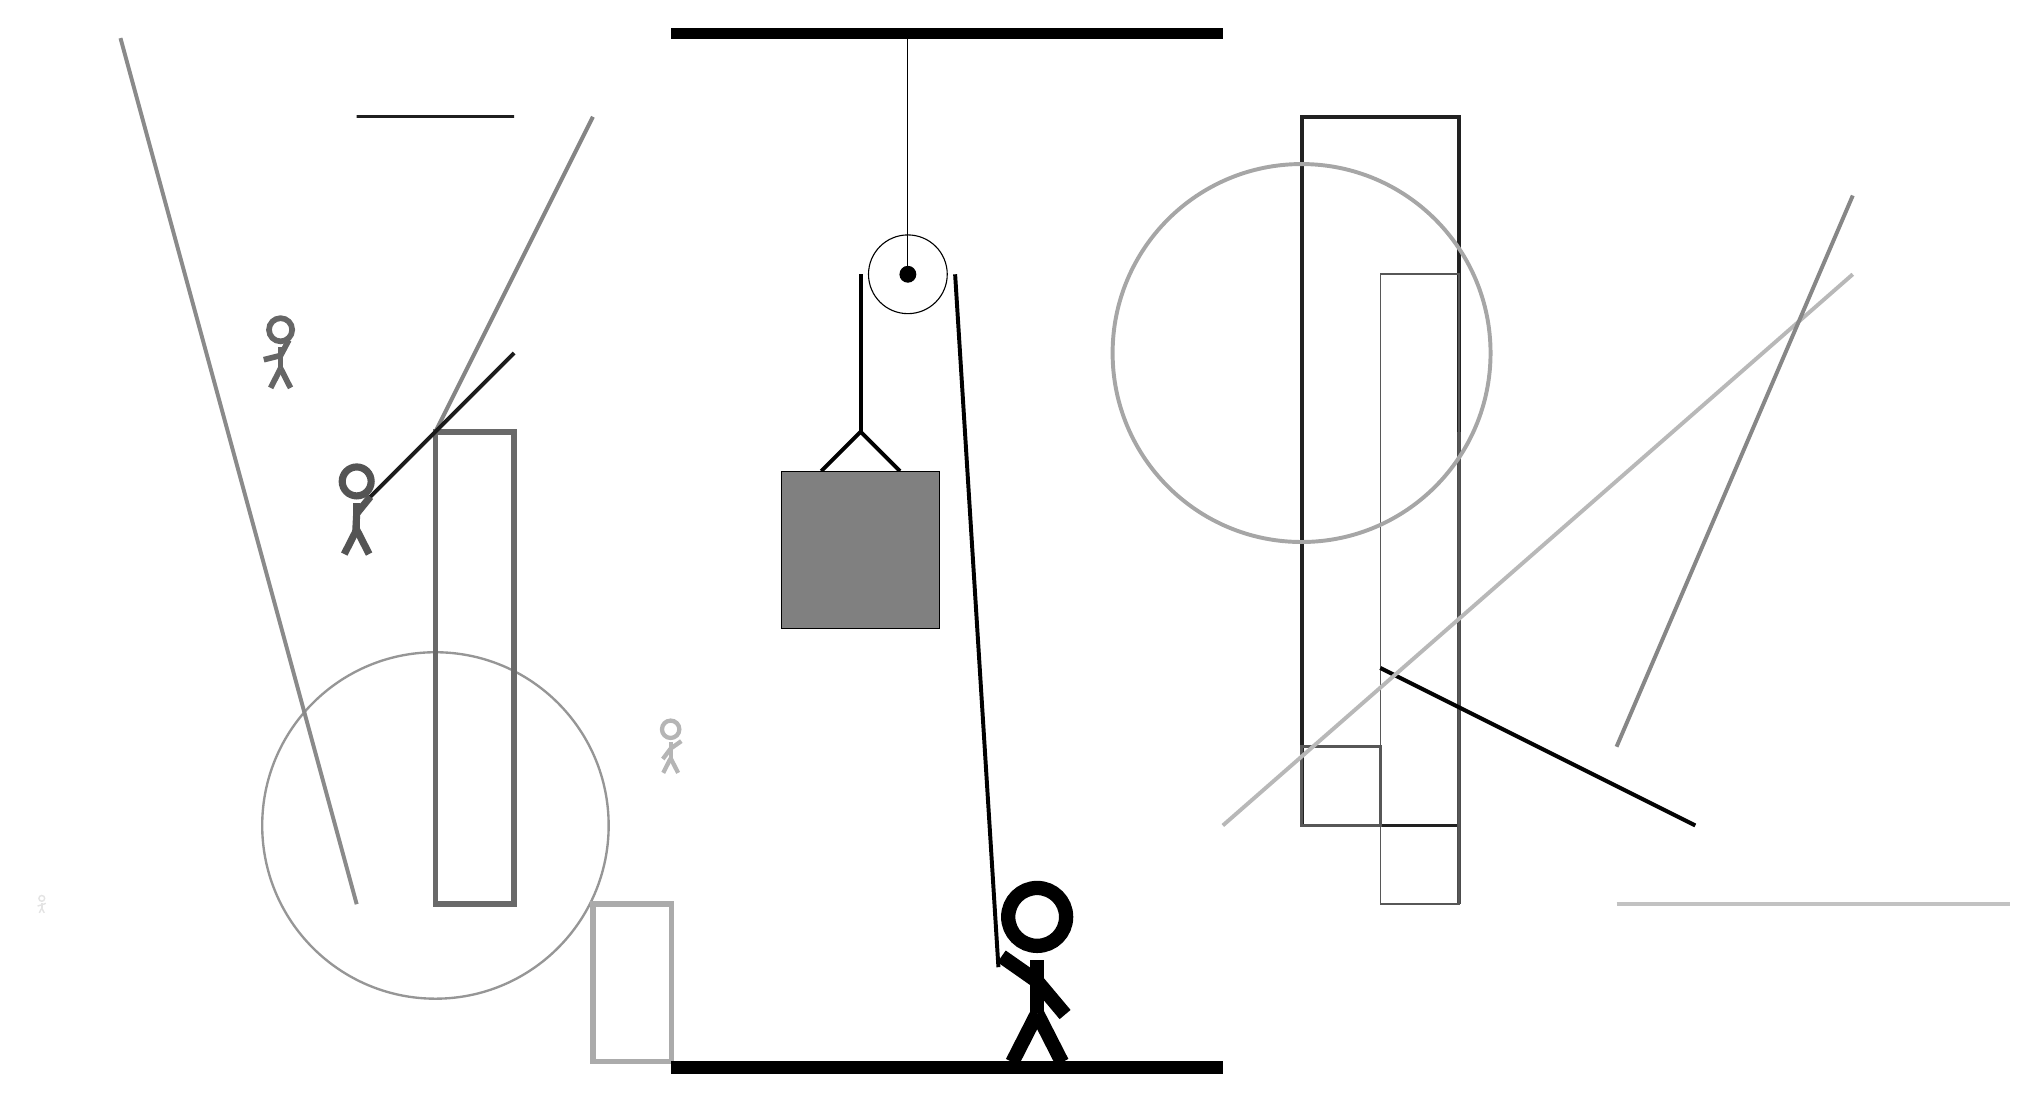
\begin{tikzpicture}
		%%%%% START %%%%%
		
		\draw[fill=black] (-2, 10) rectangle (5, 10.125);
		
		\draw (1, 7) circle (0.5);
		\draw[fill=black] (1, 7) circle (0.1);
		\draw (1, 10) -- (1, 7);
		
		\draw[line width=0.4mm, color=black!88] (-4, 9) rectangle (-6, 9);
		
		\draw[line width=0.5mm, color=black!87] (6, 0) rectangle (8, 9);
		\draw[line width=0.4mm, color=black!66] (6, 1) rectangle (7, 0);
		\draw [line width=0.3mm, color=black!41](-5, 0) circle (2.2);
		
		\draw[line width=0.5mm, color=black!70](8, -1) -- (8, 5);
		\draw[line width=0.5mm, color=black!48](-3, 9) -- (-5, 5);
		\node[line width=0.2mm, color=black!29] at (-2, 1) {\Strichmaxerl[3][53][35]};
		\draw[line width=0.2mm, color=black!66] (7, -1) rectangle (8, 7);
		\draw[line width=0.5mm, color=black!24](10, -1) -- (15, -1);
		
		\draw[line width=0.5mm, color=black!99](7, 2) -- (11, 0);
		\draw[line width=0.7mm, color=black!59] (-4, 5) rectangle (-5, -1);
		
		\node[line width=0.6mm, color=black!60] at (-7, 6) {\Strichmaxerl[4][14][62]};
		\draw[line width=0.5mm, color=black!89](-6, 4) -- (-4, 6);
		
		\node[line width=0.4mm, color=black!11] at (-10, -1) {\Strichmaxerl[1][16][20]};
		\draw[line width=0.5mm, color=black!28](5, 0) -- (13, 7);
		\draw [line width=0.5mm, color=black!35](6, 6) circle (2.4);
		\node[line width=0.5mm, color=black!67] at (-6, 4) {\Strichmaxerl[5][87][51]};
		\draw[line width=0.7mm, color=black!33] (-2, -1) rectangle (-3, -3);
		\draw[line width=0.5mm, color=black!47](10, 1) -- (13, 8);
		\draw[line width=0.5mm, color=black!46](-6, -1) -- (-9, 10);
		
		\draw[line width=0.5mm] (-0.1, 4.5) -- (0.4, 5.0) -- (0.9, 4.5);
		\draw[fill=black!50] (-0.6, 4.5) rectangle (1.4, 2.5);
		
		\draw[line width=0.5mm] (0.4, 7) -- (0.4, 5.0);
		\centerarc[line width=0.5mm](1, 7)(0:180:0.6);
		\draw[line width=0.5mm](1.6, 7) -- (2.15, -1.8);
		
		\node at (2.6, -1.9) {\Strichmaxerl[10][-35][-50]};
		
		\draw[fill=black] (-2, -3) rectangle (5, -3.15);
		
		%%%%% END %%%%%
	\end{tikzpicture}
\end{document}